\documentclass[australian,english]{article}
\usepackage[T1]{fontenc}
\usepackage[latin9]{inputenc}
\usepackage{float}
\usepackage{graphicx}
\usepackage{babel}
\begin{document}

\title{A COMP20003 Project: Unix Yelp}

\author{Luke Ceddia}
\maketitle

\section*{Introduction}

I build two programs, yelp1 and yelp2. Both perform the same operation
of querying given keys on a \foreignlanguage{australian}{CSV} file
and writing out the data found. yelp1 stores the data in a (2 branch)
binary tree, with keys equal to or less than on the left branch, and
keys greater on the right.

yelp2 uses a variant of a binary tree, using a linked list to handle
duplicates. In particular, nodes are \foreignlanguage{australian}{organised}
as per the usual method (keys less than to the left, keys greater
than to the right), but duplicates are added to a linked list originating
at the first node with that key in the tree.

\section*{Basic Operation}

The data file for each program is a series of comma-separated 'key,value'
pairs, one pair per line. This is read into memory, and the appropriate
data structure is set up. The program then reads queries from standard
input, writing results to a specified file.

\section*{Measurement}

Performance is measured with two metrics: number of key comparisons
performed for a query, and processor time (measured by clock(2)).
The former gives a machine-independent measure that is dependent only
on the algorithm; the latter allows a holistic comparison (in particular,
of the loading behaviour).

\section*{The Data}

Various files were generated, with variations on the following characteristics:
\begin{itemize}
\item Number of entries
\item Number of duplicates
\item Ordered/Randomised
\end{itemize}
The number of entries in each test database ranged from 50 to 750000
entries, with each key 40 characters long.

\section*{Experimental Results}

\subsection*{Database loading}

Both programs have similar load time behaviour; furthermore, load
time was not significantly affected by key length. In figure 1, I
plot load times for yelp1 loading a file with differing numbers of
keys.

\begin{figure}
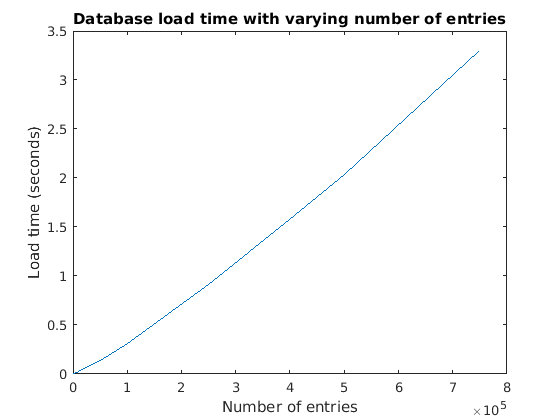
\includegraphics[scale=0.8]{figs/loadtime}

\caption{Database load time in both yelp1 and yelp2}
\end{figure}

Applying a regression to the data, the best fit is found to be $t=an^{1.2}$,
where $t$ is the load time, $n$ is the number of entries, and $a$
is a constant, not of interest here.

\subsection*{Database querying}

\subsubsection*{Number of entries: Baseline result}

To begin, I measure average key lookup times for different database
sizes. To do so, the program was fed a database of size $n$ entries,
then queried for 10\% of the entries, randomly selected. All entries
were unique, and all queries were for keys known to be in the database.
The processor time used in each query was between 3ms and 20ms. However,
it was not possible to observe any clear trends in this value. In
figure 2, I plot the average number of key comparisons performed with
each database size. The results of this test establish a \textit{baseline
result}, which other results will be compared to. By inspection, the
growth is clearly logarithmic. Note that since yelp1 and yelp2 differ
only in how they handle duplicates, the unique data produced the identical
results in both.

\begin{figure}
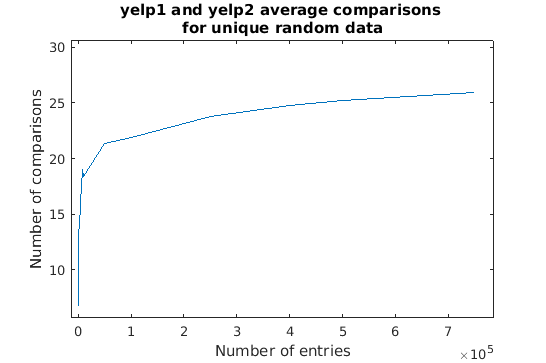
\includegraphics[scale=0.8]{figs/baseresult}

\caption{Average comparisons for query on randomised, unique data in yelp1
and yelp2 }

\end{figure}


\subsubsection*{Duplicates}

I now replace 30\% of the entries in each database with keys found
elsewhere in the file, creating duplicates. Each of these duplicate
keys is then queried, and then averaged as in the baseline test. This
result is shown in figure 3.

\begin{figure}[H]
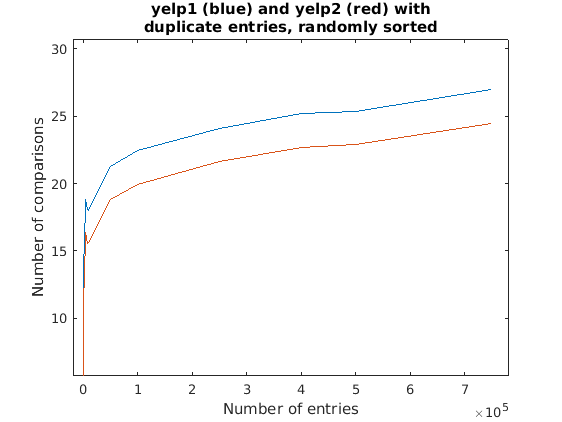
\includegraphics[scale=0.8]{figs/dups}

\caption{yelp1 (blue) and yelp2 (red) being queried for duplicated keys}
\end{figure}
Observe that while the logarithmic trend is still present, yelp2 consistently
performs fewer comparisons than yelp1 for a key with duplicate entries.
Furthermore, yelp2 performs fewer comparisons than in the baseline
test, yet yelp1 performs about the same.

\subsubsection*{Ordering}

For this test, each data file was sorted using the same comparison
function used by the programs. All entries were unique. Again comparing
number of key comparisons to number of entries, the results in figure
4 are obtained. Because of the key uniqueness, results for yelp1 and
yelp2 are again the same. Note that the behaviour is far closer to
linear than in the baseline result, with the absolute number of comparisons
being several orders of magnitudes higher.
\begin{figure}[H]
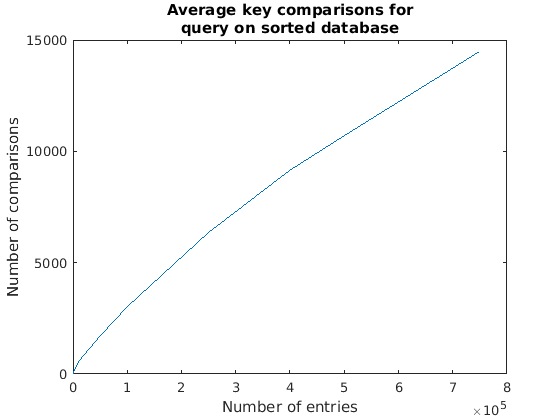
\includegraphics[scale=0.8]{figs/ordered}

\caption{Average comparisons for query on sorted, unique data. Result applies
to both yelp1 and yelp2.}

\end{figure}


\subsection*{Analysis \& Discussion}

To simplify analysis, note that yelp1 and yelp2 differ only in how
they handle duplicates. This shows why their behaviour on unique data
is the same.

\subsubsection*{Database loading}

The algorithm for loading consists of two parts: parsing and insertion.
The former has time complexity O(n), since we iterate once over each
character in the file. The latter has $nlog(n)$ time complexity in
the best case (and thus dominates over the parsing). However this
is clearly not shown in the data, where a polynomial relationship
is observed. Since the metric is processor time, there is likely a
large overhead involved in creating each node \textemdash{} the behaviour
of malloc() in particular is unknown. Since the number of duplicates
is generally small, deviation from the behaviour in the two implementations
is quite small.

\subsubsection*{Database querying}

It is known that a binary tree has $O(log(n))$ behaviour when the
data is random, allowing the tree to approximate a balanced binary
tree. The first test (figure 2) clearly demonstrates this behaviour,
with a clear logarithmic relationship between the number of entries
and number of key comparisons required. 

However, the second test (figure 3) demonstrates the difference between
yelp1 and yelp2. In yelp1, a search operation must continue down the
tree all the way to the leaf node, since a duplicate could be anywhere
along a path from the root to leaf. However, yelp2 only requires that
the first instance be located, since then the location of all other
instances are known (accessing them is a constant-time operation).
Furthermore, the number of nodes in the tree is fewer, since duplicates
do not appear. This reduces the overall depth.

This difference is evident in figure 3. The dominant factor in the
number of complexity is still the size of the dataset, but not having
to continue travelling down the tree and the depth reduction allows
yelp2 to perform better. Theoretically I would expect that the difference
between yelp1 and yelp2 would be dependent on the the fraction of
duplicates in the data, with more duplicates giving a larger gap in
the performance of the two approaches.

Finally, we examine the effect of sorting the input data. Ignoring
duplicates, inserting data in order means that the binary tree degenerates
to a linked list, with $O(n)$ lookup time. Examining test 3 (figure
4), the performance is indeed close to linear \textemdash{} extremely
close given that the same data randomised produced the strong logarithmic
relationship in figure 2. This also explains why the absolute number
of comparisons when searching sorted data is so high compared to randomised
input.

\subsection*{Conclusion}

For a key-value database, the performance of a binary tree is extremely
sensitive to the specifics of the data being handled. In particular,
sorted data results in a severe degradation of performance. The use
of a linked list to handle duplicates as done in yelp2 is a worthwhile
improvement on the standard binary tree, both helping to reduce the
overall tree size and decrease the complexity of finding all results.
The implementation would likely benefit from augmenting the binary
tree with some kind of balancing technique (such as an AVL tree),
to counteract the degenerate case of sorted data. Alternatively, a
hash table could be used in this scenario.
\end{document}
